\documentclass[11pt]{extarticle}
\usepackage{manualdoprofessor}
\usepackage{fichatecnica}
\usepackage{lipsum,media9}
\usepackage[justification=raggedright]{caption}
\usepackage[one]{bncc}
\usepackage[araucaria]{../edlab}
\usepackage{marginnote}
\usepackage{pdfpages}

\newcommand{\AutorLivro}{Arnaldo Antunes}
\newcommand{\TituloLivro}{Cultura}
\newcommand{\Tema}{Diversão e aventura}
\newcommand{\Genero}{Poesia}
%\newcommand{\imagemCapa}{./images/PNLD2022-001-01.jpeg}
\newcommand{\issnppub}{XXX-XX-XXXXX-XX-X}
\newcommand{\issnepub}{XXX-XX-XXXXX-XX-X}
% \newcommand{\fichacatalografica}{PNLD0001-00.png}
\newcommand{\colaborador}{Renier Silva}

\begin{document}

\title{\TituloLivro}
\author{\AutorLivro}
\def\authornotes{\colaborador}

\date{}
\maketitle

\tableofcontents


\begin{abstract}

Esperamos, com este material,
auxiliar os professores no trabalho com o \textbf{Ensino Fundamental \textsc{i}} em 
sala de aula. \textit{Cultura}, do poeta e compositor Arnaldo Antunes, é um livro singular
por vários motivos e possibilita atividades didáticas interessantíssimas,
como vocês acompanharão a seguir.

O poema presente nas páginas deste livro aborda, por meio de jogos linguísticos,
figuras de linguagem e as ilustrações de Thiago Lopes, 
a (re)descoberta do mundo e das coisas que o compõem. 
Os detalhes dos animais e dos elementos da natureza se organizam
para aquele que os vê, com um olhar poético, de modo particular. 
A \textit{coisa} em si nunca é simplesmente o que a palavra diz
As relações que estabelece não são as categorizadoras, que
buscam uma padronização das diferenças.
O nome de uma coisa leva a outros lugares, e a outras coisas.
É da relação entre essas descobertas que nasce o primor estético
desta poética. 

Neste manual, vocês encontrarão atividades que procuram 
trabalhar o aprimoramento do olhar poético dos alunos e alunas. 
Partimos do pressuposto muito válido de que não são só os poetas 
consagrados, como Arnaldo Antunes, que possuem tal capacidade. 
As crianças, principalmente, têm até 
uma maior liberdade na lida com o fazer poético. 
Talvez por estarem menos moldadas do que os adultos 
às convenções sociais que, na contramão do que este livro propõe,
não admitem polissemia nem criatividade entre as \textit{coisas}
e as \textit{palavras}. 

Acreditamos fortemente que o trabalho da competência linguística
e artística é essencial para a formação de um indivíduo saudável 
intelectual e socialmente. E é desta premissa que partimos para
a elaboração deste manual!

Esperamos, professores, que este material sirva como um guia 
para seu trabalho em sala de aula. Já contamos, no entanto, com as adaptações
que surgirão organicamente na recepção do mesmo por vocês, que possuem 
trajetórias e escolhas didáticas específicas, bem como no contato com os 
alunos, que tanto têm a oferecer para o enriquecimento da experiência didática.

Boa aula!

\end{abstract}

\section{Sobre o livro}

\textit{Cultura} é um livro de poesia e ilustrações que contêm o 
poema homônimo espalhado por suas páginas.
Neste poema, o mundo natural é apresentado a partir de um
ponto de vista poético. É quase como se uma criança
estivesse descobrindo pela primeira vez os animais e 
elementos da natureza e fosse nomeando as características
que veem. 
``O escuro é a metade da zebra''. ``O cavalo é pasto do
carrapato''. São formas não habituais mas válidas
e com valor estético de dar sentido ao mundo à volta.

Vale lembrar que este poema faz parte do livro \textit{As coisas}, o 
terceiro de poesia de Arnaldo Antunes. 
São ao todo 42 poemas que acompanham ``Cultura''. 

O poema inicial, ``Abertura'', serve como uma introdução ao que será
apresentado a seguir: um caráter sobretudo prosaico e narrativo.

\begin{verse}
Todos eles traziam\
sacolas, que pare-\\
ciam muito pesa-\\
das. Amarraram\\
bem seus cavalos e\\
um deles adiantou-\\
se em direção a\\
uma rocha e gritou:\\
``Abre-te, cérebro!''\\
\end{verse}

Neste poema, vemos uma referência intertextual à história de Ali Babá 
e os quarenta ladrões. Lá, Ali Babá observa a chegada, a cavalo, de
quarenta ladrões que trazem sacolas aparentemente muito pesadas. 
Param à frente de uma rocha e, para que possam adentrar na caverna do tesouro, 
devem falar as palavras mágicas: ``Abre-te, sésamo!''. Destas palavras
reverbera a abertura da porta secreta. A parte inicial do poema, narrativa, 
poderia mesmo ser retirada da história. O último verso, porém, causa 
estranheza e prepara o leitor para os poemas que encontrará no livro.

A ordem dada pelo poeta, na última linha, é: ``Abre-te, \textbf{cérebro}''. Isto serve como
uma indicação metafórica de que o cérebro se encontra fechado como uma rocha, e para
receber, ou ler, poesia necessitaria ser, ou estar, aberto e receptivo.
As ``sacolas, que pareciam muito pesadas'' podem ser entendidas, metaforicamente, como os 
poemas do próprio livro, que, no caso de o ``cérebro'' estar aberto, poderão ser descarregados e
acumulados com o restante do tesouro que se encontra guardado --- o conhecimento. 

É uma característica de Arnaldo Antunes realizar estes jogos linguísticos. 
Assim como no
poema anterior, o ludismo encontrado em ``Tudo'', na página 24, é como se fosse uma
descoberta infantil a respeito da noção da palavra homônima ao seu título:

\begin{verse}
Todas as coisas\\
do mundo não\\
cabem numa\\
ideia. Mas tu-\\
do cabe numa\\
palavra, nesta\\
palavra tudo.\\
\end{verse}

\textit{Tudo} é uma palavra que pode abarcar a totalidade das coisas ou seres. Por mais
que se queira, é praticamente impossível abarcar ``todas as coisas do mundo...numa ideia'',
mas esse vocábulo pequeno pode ser tão abrangente e genérico como o vocábulo \textit{coisa},
normalmente utilizado para indicar qualquer objeto inanimado, e por vezes animais e pessoas. 
O jogo poético reside no fato de uma ``palavra'' ter a capacidade de conter ``todas
as coisas do mundo...tudo''. É como se fosse uma descoberta, por parte de uma criança, do
poder que as palavras possuem. Esta é, aliás, uma característica constante do livro. Os
poemas funcionam como uma descoberta de mundo e das \textit{coisas} que nos cercam, como
se fossem ditas a partir do ponto de vista de uma criança, com uma linguagem simples,
direta e objetiva.


\reversemarginpar
\marginparwidth=5cm

%\marginnote{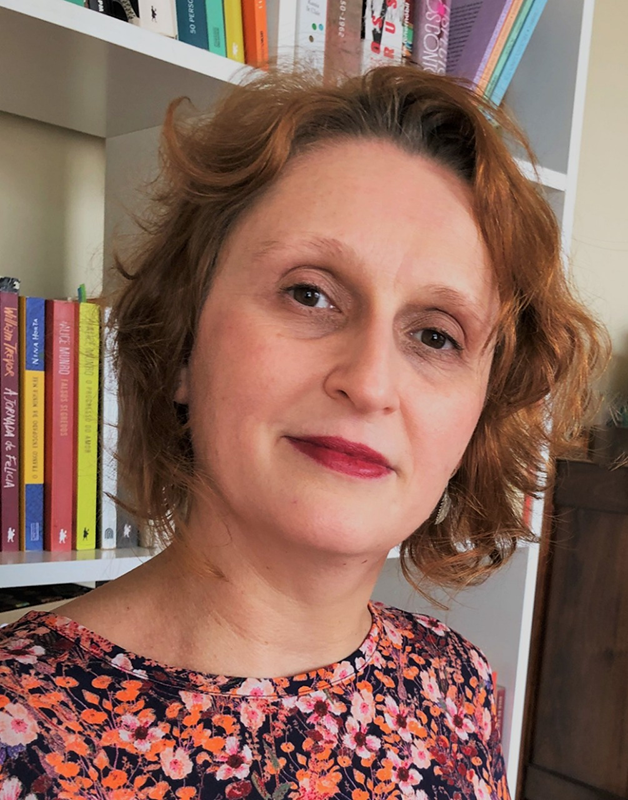
\includegraphics[width=\marginparwidth]{./images/PNLD2022-001-02.png}\\
%A autora Camila Werner (Arquivo pessoal)}


\section{Sobre o autor}


%532 caracteres
\paragraph{O autor}

\SideImage{O multiartista Arnaldo Antunes.(Foto de Jefferson Rodrigues. CC BY 2.0)}{PNLD2023-031-01.jpg}

Nascido em 2 de setembro de 1960 na cidade de São Paulo, Arnaldo Antunes é um multiartista: 
poeta, compositor, cantor popular e artista visual.
Gosta de fazer brincadeira e dar risada. Gosta de crianças e de cachorros.
Gosta de brincar com as palavras.

Nas palavras do pesquisador na área de literatura contemporânea Nielson Ribeiro Modro, 
``Arnaldo Antunes não é apenas mais um entre os muitos poetas contemporâneos''.
Seu visual alternativo e seu próprio nome sempre chamaram atenção, mas foi como poeta 
e músico que Antunes se consagrou em um
restrito grupo de artistas com destaque a nível nacional. O público que acompanha sua
produção artística varia desde jovens roqueiros até poetas consagrados de gerações anteriores, como os concretos Décio
Pignatari e Haroldo de Campos. Isto se deve ao fato de seu trabalho ser desenvolvido em
áreas distintas, porém que possuem uma íntima ligação: poesia, música e vídeo.

\begin{quote}
Percebe-se que Antunes
utiliza, em todos os seus livros, recursos oriundos de tendências literárias distintas para
construir seus poemas, principalmente advindos do Concretismo e Poesia Marginal. O uso
intencional do espaço em branco, o aproveitamento icônico, o jogo com as palavras, o
ludismo, a ingenuidade construída, a utilização de \textit{ready mades}, a originalidade, a síntese e
a objetividade podem ser apontados como características suas. Antunes consegue reunir
várias possibilidades poéticas distintas em sua obra de forma a traçar um caminho próprio;
aproveita as possibilidades existentes, mescla-as e dá-lhes características próprias e
peculiares. \footnote{\textsc{modro}, Nielson R., \textit{A obra poética de Arnaldo Antunes.} Universidade Federal do Paraná, 1996.}
\end{quote}


Entre os livros de poesia publicados, estão \emph{Psia}, \emph{Tudos}, 
\emph{As coisas}, \emph{2 ou + corpos no mesmo espaço}, \emph{Palavra desordem}, 
\emph{\textsc{et}, Eu, Tu}, \emph{N.d.a.} e \emph{Agora aqui ninguém precisa de si}, 
e livros de ensaios como \emph{40 escritos} e \emph{Outros 40}.  
Fez exposições de poesia visual em caligrafias, objetosa, vídeos, colagens e instalações. 
Como músico, lançou discos como \emph{Nome}, \emph{Ninguém} e \emph{O silêncio}.

\paragraph{O ilustrador}

Thiago Lopes nasceu em 1987 em São Paulo, onde vive, trabalha e cursa pós-graduação em 
design editorial pelo \textsc{senac}. Formou-se em design gráfico pela Faculdade Belas 
Artes de São Paulo, em 2009, com pesquisas realizadas na área de ilustração infantil e design gráfico. 
Inaugura sua carreira como ilustrador em 2010 com o lançamento do livro \textit{Junta, separa e guarda}
da autora Vera Lucia Dias publicado pela editora Callis. 

O jovem ilustrador aprendeu desde cedo a comunicar-se através da imagem e dedica-se ao universo infanto-juvenil 
com ilustrações cativantes, divertidas e delicadas.
Atualmente é sócio do Estúdio Kiwi, onde desenvolve ilustrações e projetos gráficos para 
clientes como \textsc{sesc}, \textsc{pnud}, Santander, Editora Moderna, \textsc{ftd}, 
Salamandra, Callis, Brinquebook, além da Editora Iluminuras,
da qual faz parte o presente livro.

Dentre os livros nos quais trabalhou podemos citar: 
\textit{Junta, Separa e Guarda}, \textit{\textsc{roma} -- Arte na Idade Antiga},
\textit{\textsc{egito} -- Arte na Idade Antiga}, \textit{\textsc{grécia} -- Arte 
na Idade Antiga}, \textit{Voo em português}, \textit{Tanque de Areia}, \textit{Cultura},
\textit{Poemas que escolhi para as crianças}, \textit{O Mundo da Música (Coleção com 5 volumes)},
\textit{Menina de papel}, \textit{Almanaque dos contos de fadas}, \textit{A dentadura do Seu Mokó},
\textit{Trilha na Mata}, \textit{Ai, machuquei!}, \textit{A revolta das águas}, \textit{Corrida na savana},
\textit{Os sambas dos corações partidos}, \textit{Choro e música caipira -- Ritmos do Brasil},
\textit{Carnaval -- Ritmos do Brasil}, \textit{Jovem Guarda e Tropicália -- Ritmos do Brasil},
\textit{Quer ler um livro comigo?}, \textit{Escola de príncipes encantados}, \textit{Escola de princesas recatadas},
\textit{Superligado -- Crianças na rede}, \textit{Máquinas do Tempo -- Crianças na rede},
\textit{A floresta misteriosa -- Crianças na rede}, \textit{Palavras que voam -- Crianças na rede},
\textit{As viagens da Bia}, \textit{A Bela ou a Fera}, \textit{\textsc{abc}, no labirinto da língua},
\textit{O pequeno gênio}, \textit{Almanaque da paz}, \textit{Somos parte da mudança} e
\textit{Carta à prefeita}.


\section{Sobre o gênero}

%55 caracteres
\paragraph{O gênero} O gênero deste livro é \textit{poesia}. 


Para uma primeira definição de poesia enquanto gênero literário, poder"-se"-ia recorrer à definição do professor Domingos Paschoal Cegalla, para quem ``poesia é a linguagem subjetiva, carregada de emoção e sentimento, com ritmo melódico constante, bela e indefinível como o mundo interior do poeta visa a um efeito estético''.\footnote{\textsc{cegalla}, Domingos Paschoal. \textit{Novíssima Gramática da Língua Portuguesa}. São Paulo: Companhia Editora Nacional, 2008, p.\,640}

Aprofundando um pouco essa definição, o crítico Antonio Candido expande a definição de poesia ao diferenciá"-la do verso.
Para o crítico, a poesia enquanto ato criador do artista independe da forma métrica do verso, que passa a ser apenas um dos registros possíveis do poético:

\begin{quote}
A poesia não se confunde necessariamente com o verso, muito menos com o verso metrificado. Pode haver poesia em prosa e poesia em verso livre. [\ldots]
Pode ser feita em verso muita coisa que não é poesia.\footnote{\textsc{candido}, Antonio. \textit{O estudo analítico do poema}. São Paulo: Terceira leitura, 1993, p.\,13--14.}
\end{quote}

Delineada, de forma breve e geral, a forma poética, pode"-se pensar agora em seus três gêneros básicos: lírico, épico e dramático.
Para o crítico Anatol Rosenfeld, a lírica é o gênero mais subjetivo, no qual uma voz central exprime um estado de alma traduzido em orações poéticas.
Seria a expressão de emoções e experiências vividas, ``a plasmação imediata das vivências intensas de um Eu no encontro com o mundo, sem que se interponham eventos distendidos no tempo (como na Épica e na Dramática)''.\footnote{\textsc{rosenfeld}, Anatol. \textit{O teatro épico}. São Paulo: Perspectiva, 2006, p.\,22.}

Devido a essa característica central da lírica, a expressão de um estado emocional, Rosenfeld considera que o eu"-lírico, nesse gênero, não se delineia enquanto um personagem. Embora possa evocar personagens e narrar acontecimentos, a lírica entendida enquanto gênero puro afasta"-se sobremaneira da apreensão objetiva do mundo, que não existe independente da subjetividade intensa que o apreende e exprime. Assim, na lírica prevalece a fusão entre o sujeito e o objeto, que serve mais a realçar os estados profundos de alma do poeta.
Sobre os aspectos formais do gênero, Rosenfeld nota:

\begin{quote}
À intensidade expressiva, à concentração e ao caráter ``imediato'' do poema lírico, associa"-se, como traço estilístico importante, o uso do ritmo e da musicalidade das palavras e dos versos. De tal modo se realça o valor da aura conotativa do verbo que este muitas vezes chega a ter uma função mais sonora que lógico"-denotativa. A isso se liga a preponderância da voz do presente que indica a ausência de distância, geralmente associada ao pretérito. Este caráter do imediato, que se manifesta na voz do presente, não é, porém, o de uma atualidade que se processa e distende através do tempo (como na Dramática) mas de um momento ``eterno''.\footnote{Ibidem, p.\,23.}
\end{quote}

\section{Atividades}

\subsection{Pré-leitura}

\subsubsection{Atividade 1}

\BNCC{EF05LP02}
\BNCC{EF15LP15}

\paragraph{Tema} A linguagem enquanto forma de ver o mundo. 

\paragraph{Conteúdo} Introdução à discussão a respeito da 
linguagem, apresentando-a enquanto instrumento para ver e
para modificar o mundo.

\paragraph{Justificativa} A poesia, como vimos com os autores especialistas,
está mais preocupada com a expressividade sonora da palavra e a multiplicidade
de sentidos lógicos que ela suscita. A palavra, para o poeta,
é seu instrumento de trabalho, como é o mármore para o escultor
e o violino para o músico. Elas são percebidas com cuidado e atenção
especiais. 

De forma mais simples e adequada à etapa de desenvolvimento dos alunos,
é imprescindível que eles percebam que a poesia produz imagens 
que são formas de ver o mundo diferentes da forma convencional.
Neste sentido, o olhar poético é sempre um olhar enriquecedor. 

\paragraph{Metodologia} Para introduzir o assunto, antes de chegar na poesia
propriamente, o professor ou a professora deve abordar a questão das
diferentes palavras usadas para a mesma \textit{coisa}. 
Prepare uma aula expositiva apresentando este conteúdo. 

Em diferentes idiomas uma mesma coisa é chamada de diferentes formas.
Por exemplo, o que chamamos de \textit{casa} em português, em inglês 
é \textit{house}, em francês é \textit{maison} e em tupi é \textit{oka}. 
Ainda que as palavras sejam diferentes, estão todas falando, em geral, 
da mesma \textit{coisa}: o lugar onde se mora. 

\Image{\textit{Oka} é o tipo de habitação tradicional dos povos Tupi e Guarani
que habitam o brasil. (CC BY 2.0)}{PNLD2023-031-02.jpg}

No entanto, há casos em que o que, em uma língua, é apenas \textit{uma coisa},
em outra, são várias. Por exemplo, para os povos esquimós, que vivem
numa região muito próxima ao Polo Norte e, por isso, muito fria e com
muito gelo, existem vários tipos de branco. Como boa parte das coisas
a sua volta são cobertas por gelo e neve, eles são capazes de distinguir 
uma tonalidade de outra, e o que para nós é simplesmente \textit{branco}
para eles tem bem mais sentidos. 

Para finalizar, dê um exemplo com a língua portuguesa: a palavra \textit{terra}.
\textit{Terra} pode ser aquela \textit{coisa} meio amarronzada que fica no 
chão, onde nós pisamos, onde nascem as árvores e plantas; ela pode 
ser mais firme ou mais solta, mais arenosa ou mais pedregosa.
Mas também pode ser o planeta onde vivemos, o Planeta \textit{Terra}. 
Uma mesma palavra, então, serve para expressar duas \textit{coisas} diferentes. 
O que tem uma a ver com a outra? 

Após a explicação, proponha um exercício aos alunos:

\begin{enumerate}
\item Procurem palavras que significam, assim como \textit{terra}, 
duas coisas ao mesmo tempo;

\item Depois, tentem explicar por que vocês acham que elas têm o mesmo nome:
o que elas têm em comum?

\item Compartilhem com a turma os resultados e descubra o que os seus
colegas pensaram;

\item Depois: e as palavras que são muito parecidas mas 
que não significam a mesma coisa? 

\item \textit{Casa} tem algo a ver com \textit{caça}?
\end{enumerate}

\paragraph{Tempo estimado} Duas aulas de 50 minutos.



\subsubsection{Atividade 1.2}

Dando sequência à primeira parte da atividade, na qual os alunos
começaram a perceber a riqueza do universo das palavras, 
é hora de trabalhar o aspecto da linguagem visual, também 
presente no livro por meio das ilustrações. 

Para as palavras levantadas por eles em seus exercícios,
eles devem agora, individualmente, \textbf{fazer uma ilustração},
um desenho, usando as cores e instrumentos que preferirem: lápis de cor, 
canetinha, lápis de grafite... 

Depois de feito o desenho, devem mostrá-los aos colegas.
O importante, aqui, é perceberem como, a partir da mesma 
palavra, da mesma \textit{coisa}, eles foram capazes de criar 
imagens tão diferentes. 

Por fim, encerre a etapa de pré-leitura dizendo-lhes
que \textbf{o desenho e as palavras são tipos de linguagem},
mas ainda há outros.


\subsection{Leitura}

\BNCC{EF05LP02}
\BNCC{EF35LP31}

\subsubsection{Atividade 1}

\paragraph{Tema} O que constitui um poema?

\paragraph{Conteúdo} Leitura do poema a partir de sua musicalidade e 
composição gramatical.

\paragraph{Justificativa} A leitura em voz alta de um poema é 
parte fundamental de sua experiência estética. 
É na leitura em voz alta que os aspectos sonoros
criados pelo artista e o posicionamento das
palavras na frase e no verso ganham sua potência integral. 
No caso deste poema, a musicalidade é algo que chama a atenção
e deve ser explorado pelo professor ou professora 
junto à turma. 

Gramaticalmente, as classes das palavras podem ser trabalhadas
pensando nas classificações das rimas em \textbf{ricas} e \textbf{pobres},
sendo as primeiras, aquelas entre palavras de classes diferentes,
e as segundas, entre palavras de classes iguais. 

\paragraph{Metodologia} Faça uma leitura em voz alta do poema.
Depois, peça para que alguns alunos e alunas leiam, 
sempre em voz alta.
Chame a atenção para a sonoridade do poema e os aspectos formais
das \textbf{rimas}, como em \textit{sapo/\,papo/\,gato\,pasto\,carrapato}, \textit{novo/\,ovo/\,corpo/\,porco} e
\textit{ganso/\,manso/}, além de outras.

\begin{itemize}
\item Quais são as palavras que rimam? 
\item A quais classes elas pertencem?
\end{itemize}

Apresente, então, algumas das classes gramaticais das 
palavras em português.
Os \textbf{substantivos}, por exemplo, são palavras utilizadas
para dar nome aos seres, objetos, sentimentos, cores, entre outros.
Já os \textbf{adjetivos} servem para caracterizar os substantivos,
ou seja, atribuir-lhes qualidades positivas, negativas ou neutras. 
Os adjetivos sempre concordam em gênero e número com os substantivos!
Outra classe gramatical existente é a dos \textbf{numerais} que, como
o nome indica, servem para quantificar algo, definindo seu valor numérico. 
Os \textbf{pronomes} acompanham ou representam um substantivo.
Os \textbf{verbos} expressam uma ação, um estado, um desejo,
um acontecimento ou um fenômeno natural. Os verbos variam de acordo
com a pessoa que fala, ou seja, se se trata da primeira pessoa
do singular, ele terá uma forma; se se trata da primeira pessoa do
plural, terá outra. 
Os \textbf{advérbios}, por fim, servem para qualificar os verbos e adjetivos,
complementando seus sentidos.

Apresente, então, uma lista de exemplos para cada classe:

\begin{itemize}
	\item Substantivos: fogo, água, João, Maria, Brasil, escola...
	\item Adjetivos: quente, molhada, bonito, inteligente, grande, esperto...
	\item Numerais: um, dois, primeiro, segundo, metade, dobro, triplo...
	\item Pronomes: ele, ela, nós, a gente, meu, nosso, aquela, onde...
	\item Verbos: adorei, conversamos, é, são, digitam, adorar, ser...
	\item Advérbios: bem, mal, muito, pouco, lentamente, rapidamente...
\end{itemize}

Por fim, peça que os alunos e alunas adicionem à
lista de exemplos as palavras que compõem o poema.
Depois, eles devem procurar as palavras que rimam e, 
então, classificá-las de acordo
com suas classes gramaticais. Assim, poderão dizer
se se trata de rimas ricas ou pobres. 

\paragraph{Tempo estimado} Quatro aulas de 50 minutos.

\subsubsection{Atividade 2}

\BNCC{EF01CI03}

\paragraph{Tema} As ciências e a poesia. 

\paragraph{Conteúdo} Noções gerais sobre as classificações
dos seres vivos e relação com a poesia. Desmistificação da
ideia de que toda bactéria é ruim. Definição de cultura.

\paragraph{Justificativa} A ciência existe como uma faculdade 
que procura classificar e explicar as coisas existentes no mundo
e para além dele. Por isso, ela precisa ser clara e objetiva.
A poesia, no entanto, não trabalha necessariamente com esta
mesma obrigação. Ainda assim, ou até mesmo por conta disso,
as relações entre estas duas áreas da produção do conhecimento
humana sejam tão frutíferas quando trabalhadas em conjunção. 
É importante que alunos e alunas percebam a arte como 
uma forma de conhecimento e expressão que não invalida a ciência,
mas que convive com ela, completando-a, incentivando-a,
ilustrando-a e o que mais for do gosto do artista. 

\paragraph{Metodologia} Comece a aula com as duas perguntas
que serão centrais para o desenvolvimento da atividade:

\begin{itemize}
\item O que são bactérias?
\item O que é cultura?
\end{itemize}

Após o levantamento de respostas, que devem ser anotadas na lousa,
apresente uma definição científica dos dois termos.
Bactérias são seres vivos muito pequenos que estão espalhados
por todos os lugares do planeta. 
Mesmo dentro de nosso corpo existem
bactérias. Por exemplo, em nosso intestino existem bactérias
responsáveis por transformar os alimentos que consumimos
em nutrientes para nosso corpo. Um exemplo são os lactobacilos vivos presentes
no leite fermentado que tomamos, que fazem parte do que chamamos de \textbf{flora intestinal}.
Por outro lado, existem as bactérias que fazem mal para a saúde humana,
causando doenças e até podendo levar à morte. É o caso dos bacilos 
que causam tuberculose, lepra, disenteria, entre outras. 

Em todo caso, sejam elas benéficas ou maléficas à saúde humana, 
as bactérias nunca estão sozinhas, como acontece com outros tipos
de seres vivos. Elas estão sempre em comunidades que recebem o
nome de \textbf{cultura}.

\Image{Reprodução de página do livro dedicada às bactérias.}{PNLD2023-033-02.jpg}

A palavra cultura tem origem no latim \textit{colere}, que significa 
cuidar, cultivar e crescer. Cultura, portanto, é tudo
aquilo que seres vivos fazem para cultivar suas vidas,
fazendo-as crescer e se manter vivas. 

No caso dos seres humanos, cada povo tem uma cultura diferente,
e nenhuma delas é mais importante ou mais verdadeira do que a outra,
afinal, todos os povos têm o direito de existir e cultivar a vida. 
A língua, a religião, as linguagens artísticas como a música,
a poesia, a dança e o teatro, a arquitetura, enfim... muito 
do que possivelmente foi levantado pela turma. 

Cultura, então, é algo bom. Por isso ``bactérias num meio é cultura''.

Após a exposição sobre \textbf{bactérias} e \textbf{cultura},
releiam juntos o livro em voz alta. 

\paragraph{Tempo estimado} Duas aulas de cinquenta minutos.


\subsection{Pós-leitura}

\subsubsection{Atividade 1}

\BNCC{EF15AR24}
\BNCC{EF03ER03}
\BNCC{EF03LP13}

\paragraph{Tema} Oficina de criação poética, visual e musical.

\paragraph{Conteúdo} Produção musical e visual a partir de um poema.

\paragraph{Justificativa} A interdisciplinaridade artística é elemento
constitutivo do trabalho de Arnaldo Antunes. De certa forma, 
é impossível dissociar seus versos escritos dos versos cantados
ou grafados em seus vídeos. Por isso, a recepção de seu trabalho
não pode deixar de levar em conta este aspecto, não apenas
na apreciação passiva, como na experimentação do processo
da parte dos alunos. 

\paragraph{Metodologia} Inicie a aula pedindo que os alunos
escrevam um poema inspirados no livro que leram.
Eles devem levar em conta a sonoridade, as rimas, e sobretudo
o olhar poético, aquele que busca criar relações de sentido
entre as coisas físicas ou abstratas. 

Paralelamente à criação dos versos, eles devem criar ilustrações para 
os mesmos com instrumentos como canetinha colorida, lápis de cor,
lápis de grafite ou mesmo tinta; o que estiver disponível na escola. 

Mostre aos alunos algumas músicas de Arnaldo Antunes feitas a partir de
poemas do livro \textit{As coisas}, como ``As coisas'', ``Cultura'' e
``O fogo''. Os links estão indicados nas \textbf{Sugestões de referências complementares}.

Então, é a vez dos alunos \textbf{criarem} uma música a partir dos poemas.
O mais importante, aqui, é deixar claro que não há uma ordem
correta para o trabalho: eles podem começar escrevendo os versos
e partir para o desenho e, depois, para a música, ou o contrário. 
O que importa é que as três coisas estejam juntas e façam sentido entre si.

Eles podem trabalhar em grupos ou individualmente,
conforme a melhor disposição da turma. 
Ao fim, é interessante que seus trabalhos sejam compartilhados
com a turma e, eventualmente, com as outras turmas da escola.

\paragraph{Tempo estimado} Quatro aulas de 50 minutos.


\section{Sugestões de referências complementares}

\paragraph{Música}

\begin{itemize}
\item \href{https://www.youtube.com/watch?v=JF4MruZSwzg}{``As coisas''}. Música de Arnaldo Antunes do álbum \textit{Qualquer}, de 2006.  

\item \href{https://www.youtube.com/watch?v=Aguu_QzCQy8}{``Cultura''}. Música de Arnaldo Antunes do álbum \textit{Nome}, de 1993.  

\item \href{https://www.youtube.com/watch?v=kUgUNHj2VlE}{``O fogo''}. Música de Arnaldo Antunes do álbum \textit{Disco}, de 2015.  
\end{itemize}


\paragraph{Livros e artigos}
% Comentário de Rogério: os livros abaixo são a respeito de cordel. Não é o caso de alterar essa bibliografia?

\begin{itemize}
\item \textsc{daghlian}, Carlos (org.). \textit{Poesia e música / Debates 195}. São Paulo: Perspectiva, 1985.

\item \textsc{modro}, Nielson Ribeiro. \textit{A obra poética de Arnaldo Antunes}. Dissertação de Mestrado em Letras. 
Universidade Federal do Paraná, 1996.

\item \textsc{pignatari}, Décio. \textit{O que é comunicação poética}. São Paulo: Brasiliense, 1991.

\item \textsc{sant'anna}, Afonso Romano de. \textit{Música popular e moderna poesia brasileira}. Petrópolis: Vozes, 1977.

\item \textsc{tatit}, Luiz. \textit{A canção: eficácia e encanto}. São Paulo: Atual, 1986.
\end{itemize}

\section{Bibliografia comentada}

\begin{itemize}
\item \textsc{brasil}. Ministério da Educação. \textit{Base Nacional Comum Curricular}. Brasília, 2018.

Consultar a \textsc{bncc} é essencial para criar atividades para a turma. Além de especificar 
quais habilidades precisam ser desenvolvidas em cada ano, é fonte de informações sobre 
o processo de aprendizagem infantil. 

 \item \textsc{porto}, Paulo Alves. \href{http://qnesc.sbq.org.br/online/qnesc11/v11a07.pdf}{``Augusto dos 
 	Anjos: Ciência e Poesia''}. Revista \textit{Química Nova na Escola},
	nº 11, maio de 2000.  

No presente artigo pretende-se mostrar como o conhecimento de ciências em geral (química e biologia em
particular), e de sua história, pode contribuir para a fruição estética de um poema.


\item \textsc{van der linden}, Sophie. \textit{Para ler o livro ilustrado}. São Paulo: Cosac Naify, 2011.

Livro sobre as particularidades do livro ilustrado, que apresenta as diferenças entre o livro ilustrado e o livro com ilustração. 
\end{itemize}

\end{document}